\chapter{Graph Layout Algorithms}

Graph layout algorithms (or GLAs for short) are a class of algorithms used for computing positions
of nodes so that they make a nice or useful diagram.
These algorithms accept graph-representing data as input and produce positions of individual nodes as output.

In this work, we are going to assume that GLAs produce 2-dimensional layouts,
but it is worth mentioning that the number of dimensions can be arbitrarily high.

There are many types of GLAs, each with its own strengths and weaknesses. Let'S look at some of the common ones.

\section{Circular Layout}

Circular layout (figure \ref{obr:graph_layout_circular}) algorithms arrange nodes in a circle, often emphasizing the structure of the graph by placing nodes
with similar properties close together.
In a circular layout, nodes can be distributed evenly along the circumference of the circle,
or their placement can be weighted by certain properties (e.g., node degree or importance).

\begin{figure}[p]\centering
    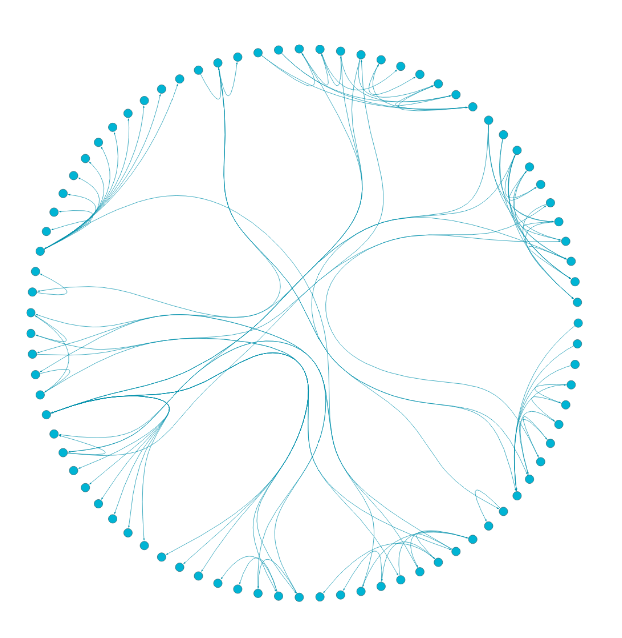
\includegraphics[width=140mm, keepaspectratio]{img/graph_layout_cicrular.png}
    \caption{Circular layout\cite{graph_layout_demos}}
    \label{obr:graph_layout_circular}
\end{figure}

\section{Hierarchical Layout}

Hierarchical layout (figure \ref{obr:graph_layout_hierarchical})algorithms are designed to emphasize directional relationships, such as those found in flowcharts,
dependency graphs, or organizational charts. These algorithms arrange nodes in layers or levels, with edges generally
flowing in a single direction (e.g., top to bottom or left to right).
This layout can be applied to general graphs but is most effective for directed acyclic graphs (DAGs) or undirected trees.

\begin{figure}[p]\centering
    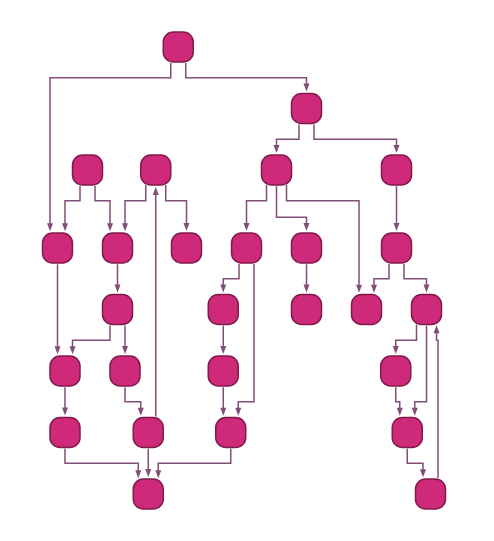
\includegraphics[width=140mm, keepaspectratio]{img/graph_layout_hiearchichal.png}
    \caption{Hierarchical layout\cite{graph_layout_demos}}
    \label{obr:graph_layout_hierarchical}
\end{figure}

\section{Radial Layout}

Radial layout (figure \ref{obr:graph_layout_radial}) is a type of hierarchical layout where nodes are arranged in concentric circles around a central node.
Its immediate neighbors are arranged in the first circle. Subsequent layers represent nodes further away.
Radial layout can help highlight relationships between the central node and its surroundings.

\begin{figure}[p]\centering
    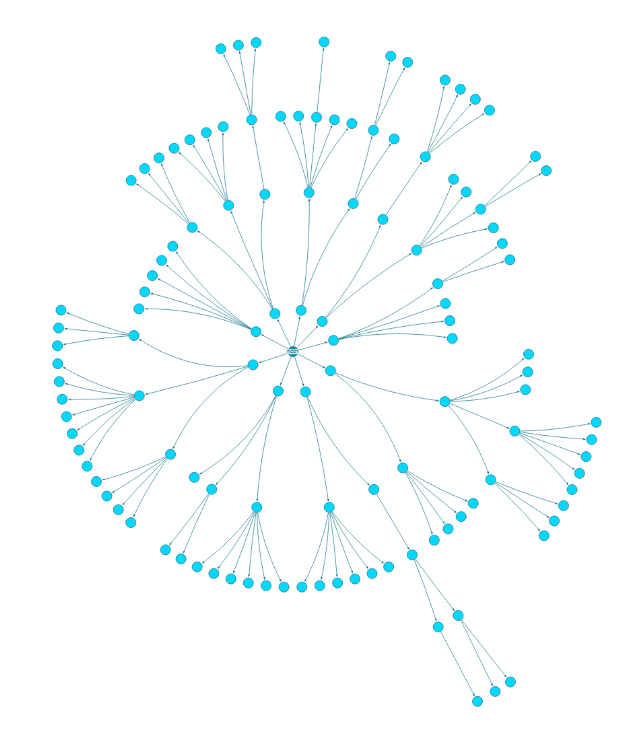
\includegraphics[width=140mm, keepaspectratio]{img/graph_layout_radial.png}
    \caption{Radial layout\cite{graph_layout_demos}}
    \label{obr:graph_layout_radial}
\end{figure}

\section{Force-Directed Layout}
All graph layouts we saw in chapter 1 were produced by force-directed layout (FDL) algorithms.
\footnote{We weren't able to find any specifics about the algorithm used in Obsidian.
However, from the way its graph view behaves, it is safe to assume a variation of an FDL algorithm was used.}

The main idea behind FDL algorithms is very intuitive:
nodes are attracted to each other when connected by an edge and repelled otherwise.
Elegant in concept and easy to implement, this approach is endlessly customizable.

One particularly useful feature is that FDL algorithms are incremental and update the layout continuously.
This can be utilized to produce visually pleasing animations of the data and allows for user interaction
(e.g., dragging nodes around or changing parameters).
The draging feature can also be used to aid the layout algorithm towards a more desired layout.

Thanks to this aspect, a developer implementing an FDL algorithm has the ability to adjust the strength of the forces, add new ones,
or implement entirely new behaviors and parameters to fit specific use cases 
- all by watching the animation run, interacting with it and inferring what behavior needs to be changed or added.

These positives are, however, balanced by two drawbacks:
\begin{itemize}
    \item high time complexity

    The basic version of FDL has a time complexity of $O(n^2)$ per step, where $n$ is the number of nodes in the graph.
    For stabilization, usually $n$ steps are considered sufficient,
    and thus the time complexity for producing a stabilized graph is often computed as $O(n^3)$.

    \item sensitive parameterization
    
    As for parameterization, the algorithm is highly dependent on the parameters set by the user (or developer),
    some of which can be very sensitive and radically change the resulting layout with only a small change in value.
    This can be a challenge for users who are not familiar with the algorithm or the data they are working with.
    Achieving a specific look or quality for the final graph render often requires time spent tweaking the parameters.
\end{itemize}